\documentclass{beamer}
\usepackage[galician]{babel}
\usepackage[utf8x]{inputenc}
\usepackage{fontenc}
\mode<presentation>{\usetheme[secheader]{Boadilla}}

\title{Obradoiro de introdución a Arduino}
\author[Brais, Rafa, Tucho]{ Brais Arias \\ Rafa Couto \\ Tucho Méndez}
\date{2014-10-08}

\begin{document}

\begin{frame}
\titlepage
\begin{center}
\begin{columns}
\begin{column}{0.33\textwidth}
\begin{center}

\includegraphics[width=50pt]{./img/bricolabs.png}
\end{center}
\end{column}

\begin{column}{0.33\textwidth}
\begin{center}

\includegraphics[width=50pt]{./img/gpul.png}
\end{center}
\end{column}

\begin{column}{0.33\textwidth}
\begin{center}

\includegraphics[width=50pt]{./img/licencia.png}
\end{center}
\end{column}
\end{columns}
\end{center}
\end{frame}

%% Indice de contidos
\begin{frame}{Indice}
  \tableofcontents
\end{frame}

%%%%%%%%%%%%%%%%%%%%%%%%%%%%%%%%%%%%%%%%%%%%%%%%%%%%%%
\section{Hardware Libre}
\begin{frame}
\huge{\centerline{\textbf{\color{blue} \insertsection}}}
\end{frame}

% % % % % % % % % %
\begin{frame}
\begin{itemize}
\item Similar ao Software Libre e Coñecemento Libre.
\item Deseño dipoñíbel para:
\begin{itemize}
 \item Estudar
 \item Modificar
 \item Distribuir
 \item Materializar
\end{itemize}
\end{itemize}

\begin{center}

\includegraphics[width=150pt]{./img/Ohw-logo.png}
\end{center}


\end{frame}

% % % % % % % % % %
\begin{frame}{Proxectos Hardware Libre}

\begin{columns}
\begin{column}{0.25\textwidth}
\begin{itemize}
\item Aurora
\item Uze
\item Arduino
\item Reprap
\item ...
\end{itemize}
\end{column}
\begin{column}{0.75\textwidth}

\begin{columns}
	\begin{column}{0.35\textwidth}
		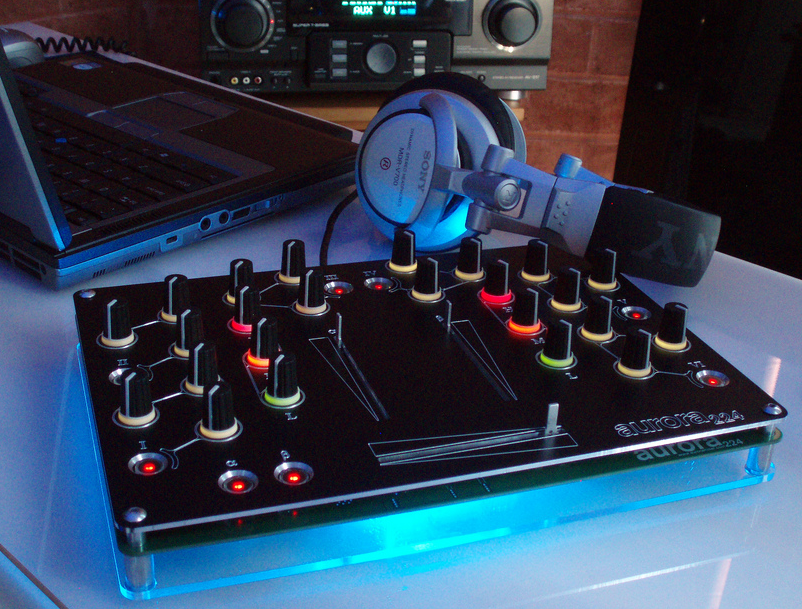
\includegraphics[width=100pt]{./img/exemplo_Aurora.png}

		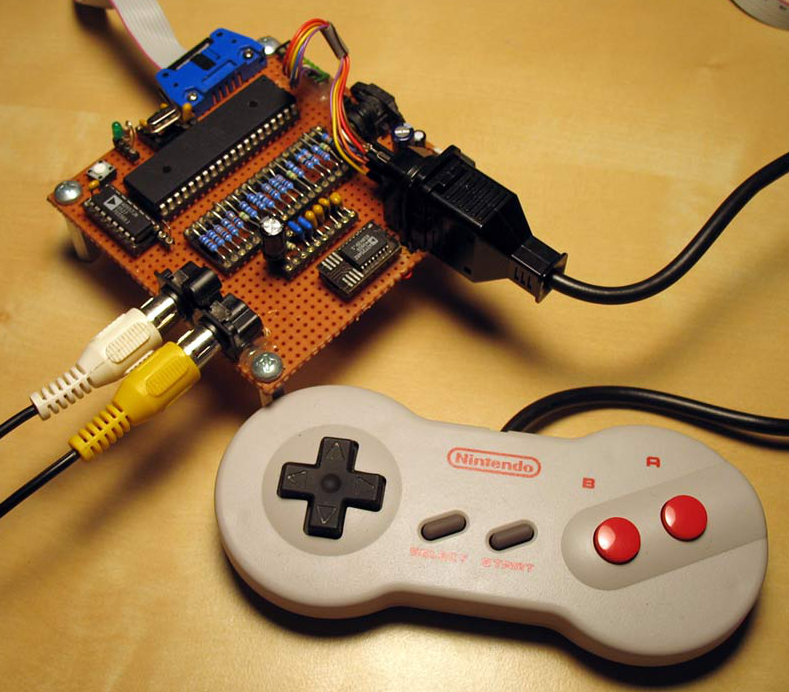
\includegraphics[width=100pt]{./img/exemplo_Uze.png}
	\end{column}
	\begin{column}{0.35\textwidth}
		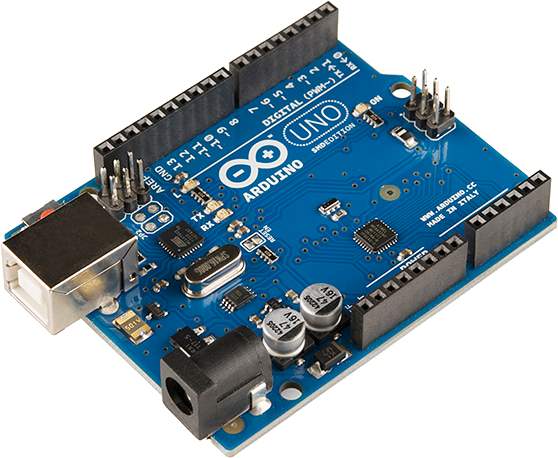
\includegraphics[width=100pt]{./img/Arduino_Uno.png}

		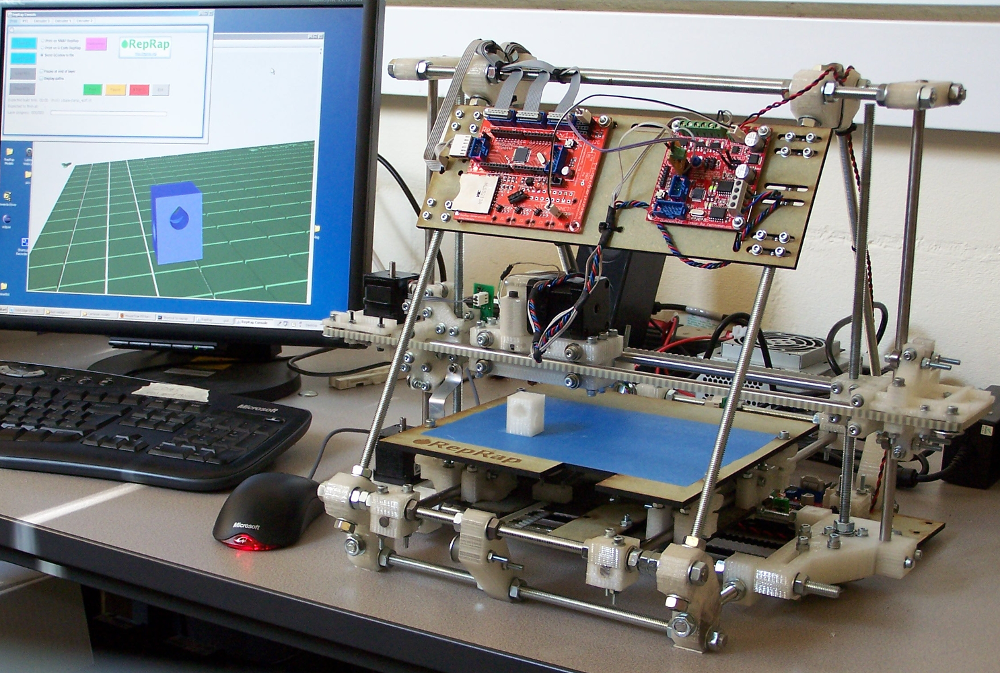
\includegraphics[width=100pt]{./img/exemplo_RepRap_v2_Mendel.png}
	\end{column}
\end{columns}

\end{column}
\end{columns}


\end{frame}


%%%%%%%%%%%%%%%%%%%%%%%%%%%%%%%%%%%%%%%%%%%%%%%%%%%%%%
\section{Arduino}
\begin{frame}
\huge{\centerline{\textbf{\color{blue} \insertsection}}}
\end{frame}


% % % % % % % % % %
\begin{frame}{Que é Arduino?}
\begin{columns}
\begin{column}{0.5\textwidth}
	\begin{itemize}
	\item Placa de prototipado eletrónico
	\item Hardware Libre
	\item Orixinario en 2005 en Italia por artistas
	\item David Cuartielles e Massimo Banzi
	\end{itemize}
\end{column}
\begin{column}{0.5\textwidth}
	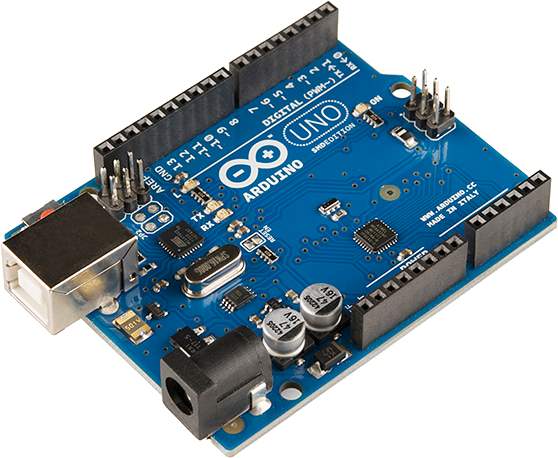
\includegraphics[width=150pt]{./img/Arduino_Uno.png}
\end{column}
\end{columns}

\end{frame}

% \begin{frame}
%
% \end{frame}

% % % % % % % % % %
\begin{frame}{Que máis é Arduino?}
\begin{itemize}
 \item Non solo placas controladoras
 \item IDE (Entorno de Desenvolvemento)
 \item Liguaxe de programación
 \item Comunidade (playground.arduino.cc, bricolabs \dots)
\end{itemize}

\end{frame}

% % % % % % % % % %
\begin{frame}{Arquitectura}
\begin{columns}
	\begin{column}{0.4\textwidth}
		\begin{itemize}
			\item Microcontrolador ATmega
			\item Reloxo
			\item Controlador USB (non todos)
			\item Entradas e saidas (pines)
			\item EEPROM
		\end{itemize}
	\end{column}
	\begin{column}{0.6\textwidth}
		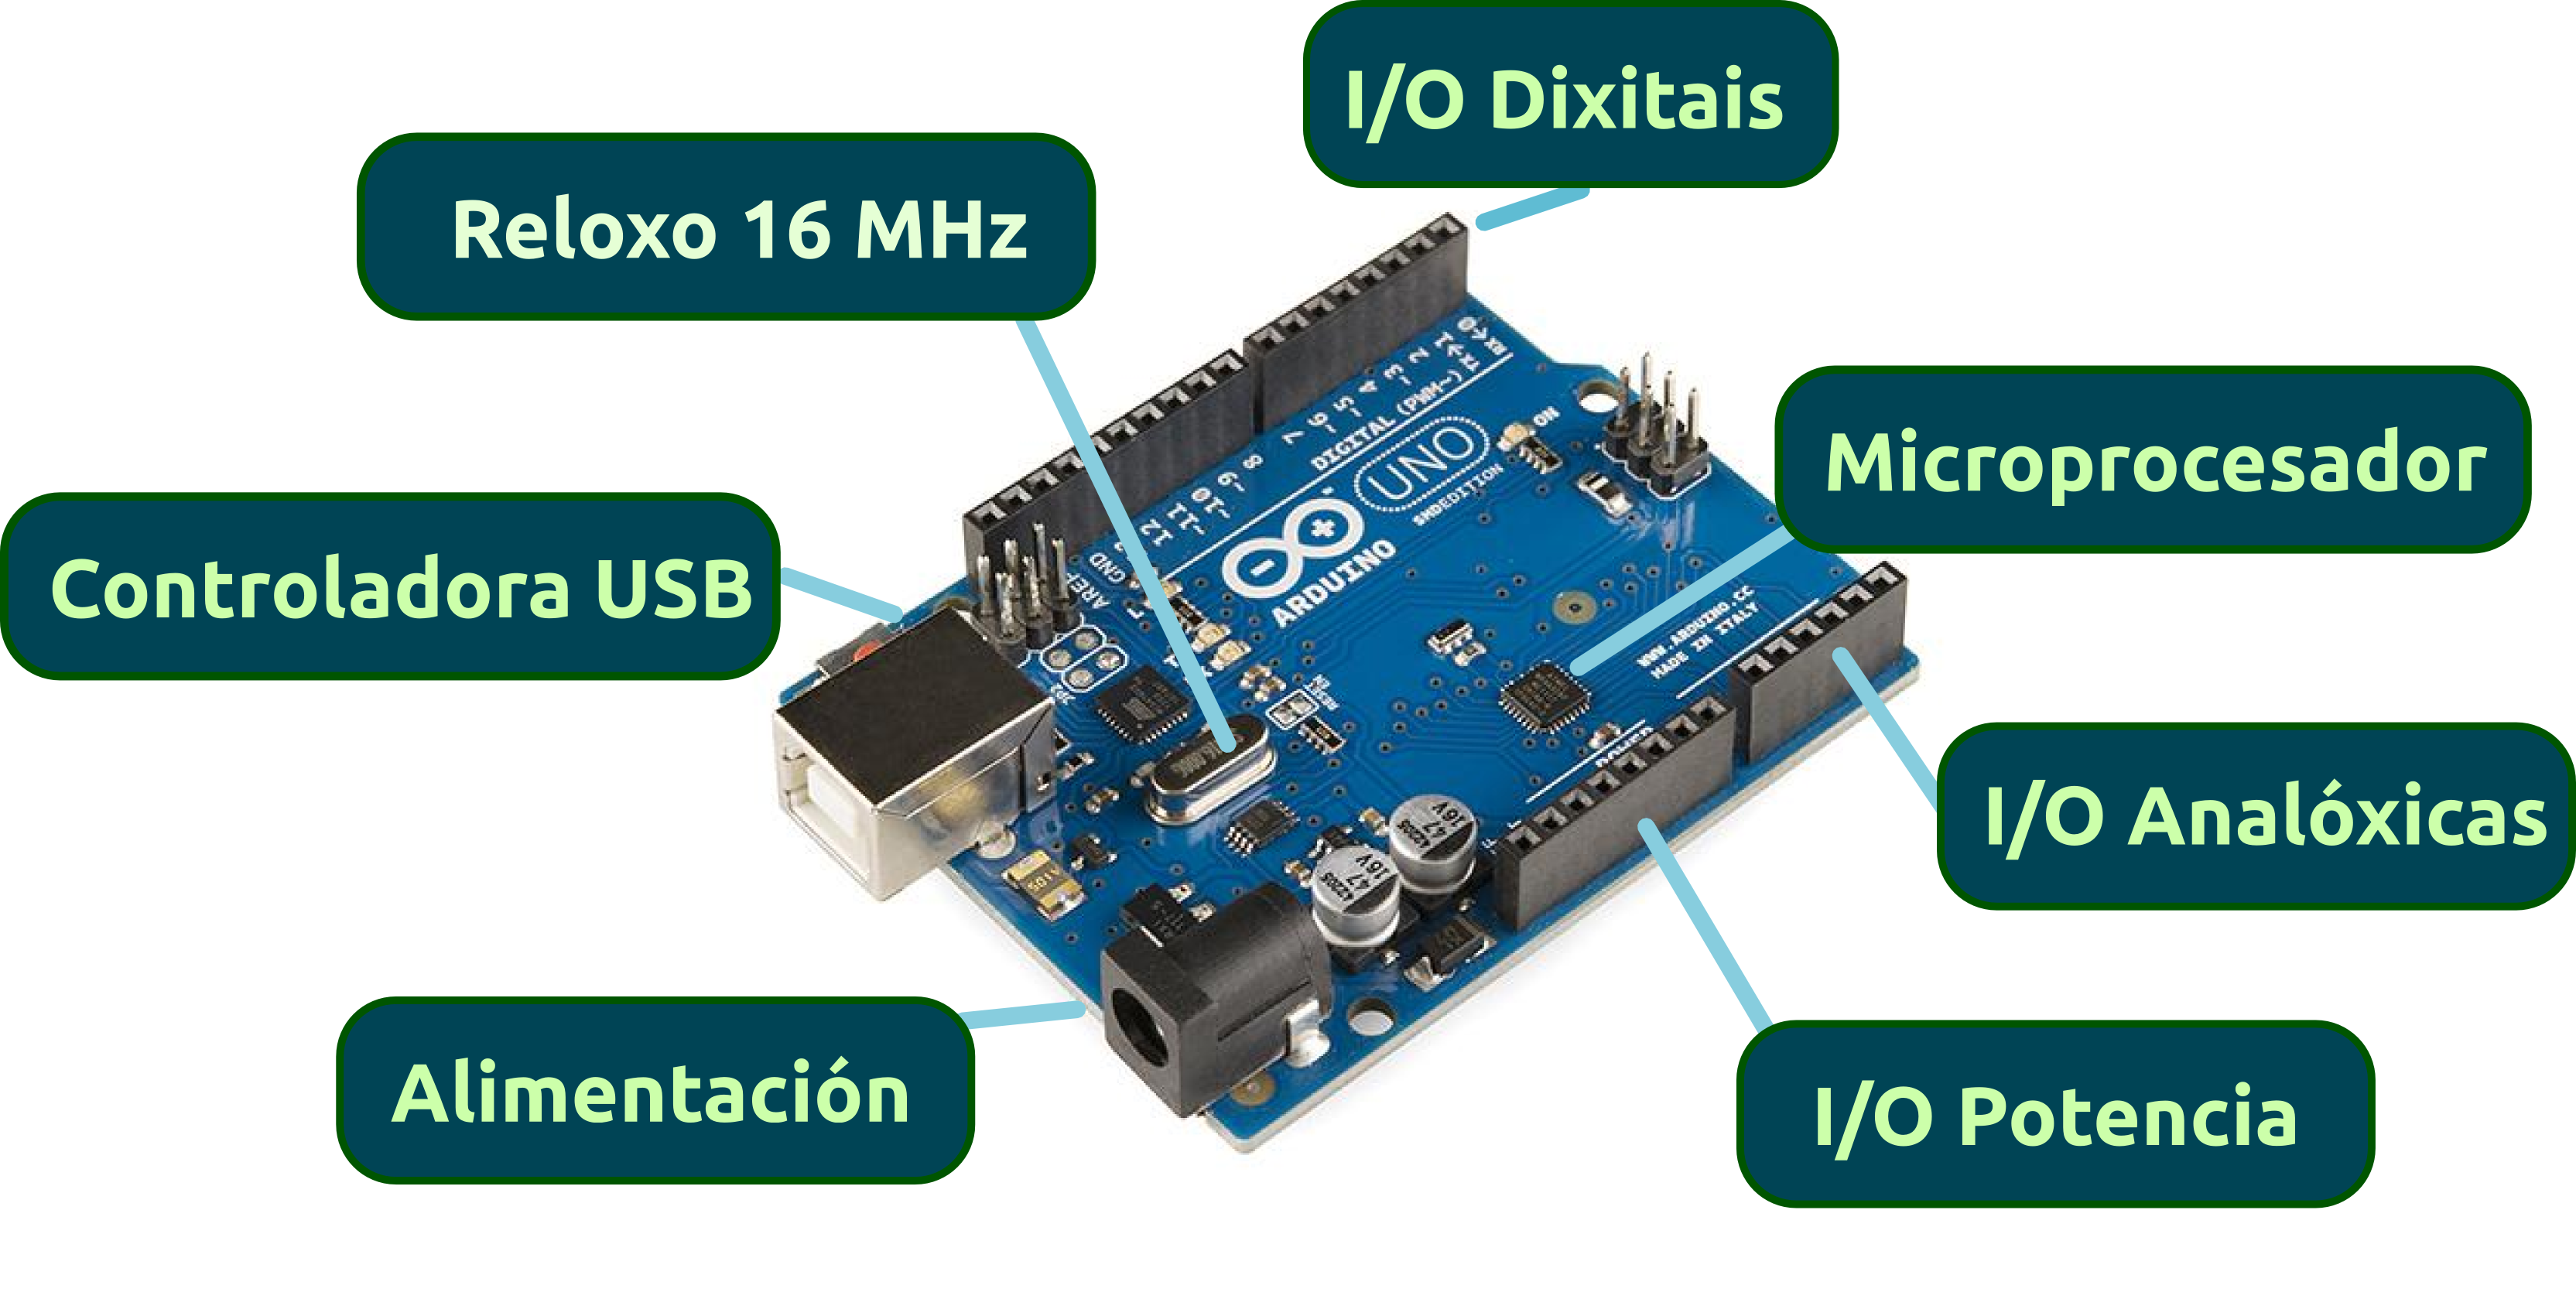
\includegraphics[width=200pt]{./img/arduinoUNOExplicado.png}
	\end{column}
\end{columns}
\end{frame}



% % % % % % % % % %
\begin{frame}{Variedades}

\begin{columns}
\begin{column}{0.25\textwidth}
\begin{itemize}
\item Placas
\begin{itemize}
\item UNO
\item Mega
\item Pro
\item Micro
\item Fio
\item Robot
\item LilyPad
\item ...
\end{itemize}
\item Shields
\begin{itemize}
\item Xbee
\item Motor Control
\item Wifi
\item Ethernet
\item ...
\end{itemize}
\end{itemize}
\end{column}

\begin{column}{0.75\textwidth}
\begin{columns}
\begin{column}{0.55\textwidth}
\begin{center}
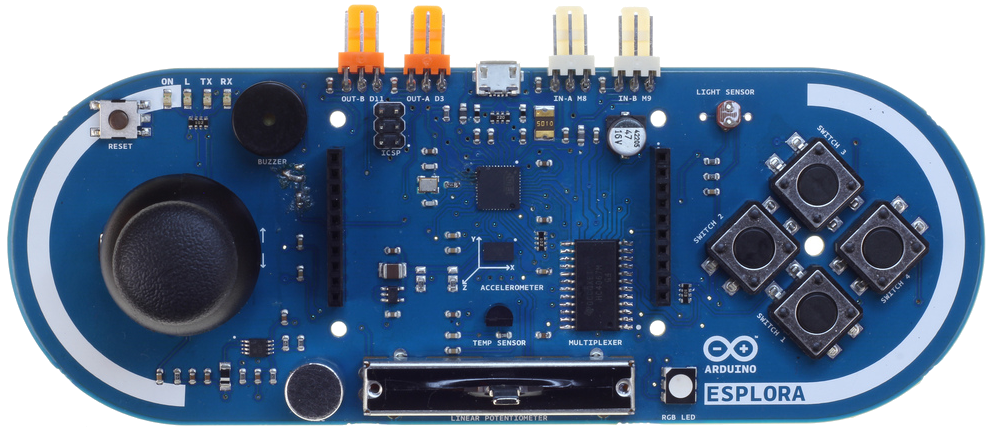
\includegraphics[width=100pt]{./img/arduino_esplora.png}


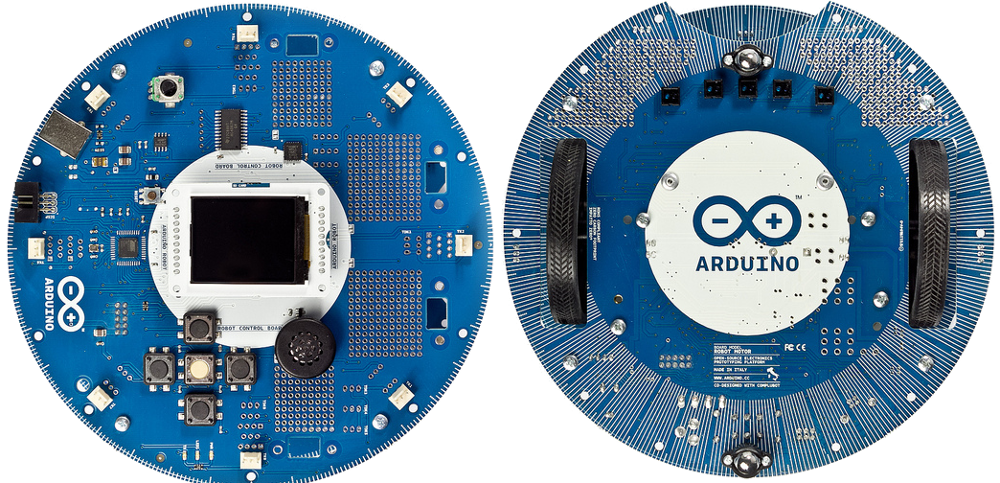
\includegraphics[width=150pt]{./img/arduino_robot.png}


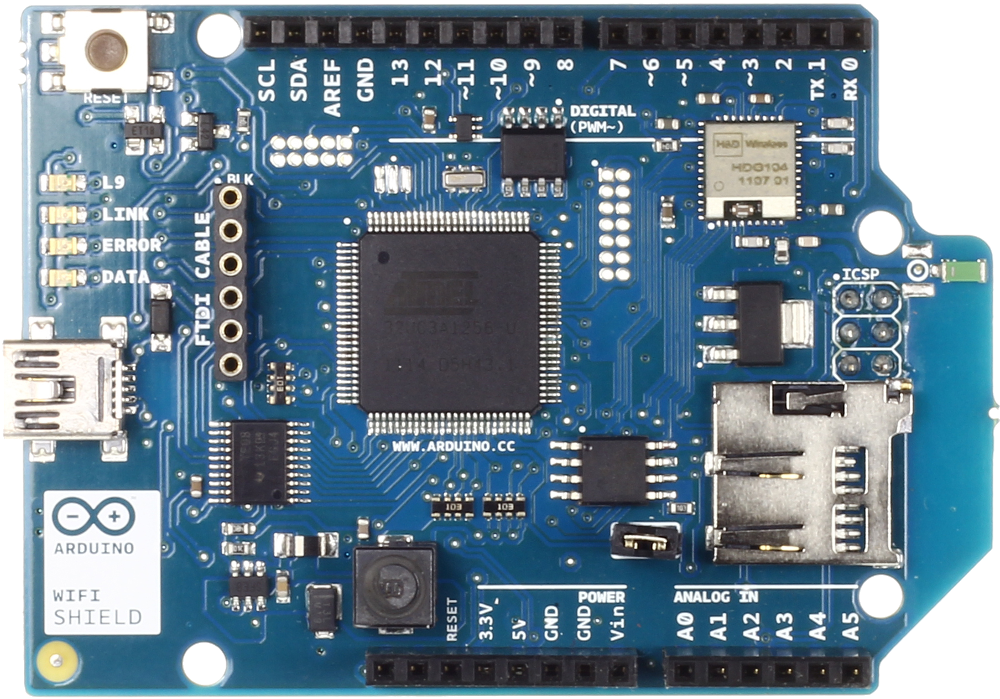
\includegraphics[width=100pt]{./img/shield_wifi.png}
\end{center}
\end{column}
\begin{column}{0.2\textwidth}
\begin{center}
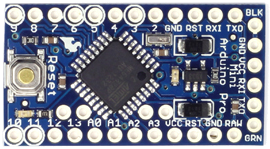
\includegraphics[width=50pt]{./img/arduino_pro_mini.png}


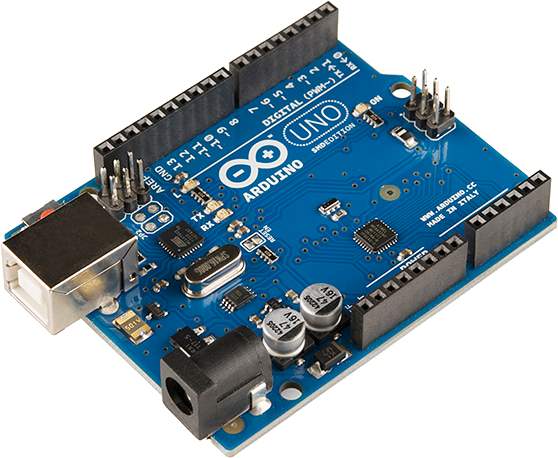
\includegraphics[width=70pt]{./img/Arduino_Uno.png}


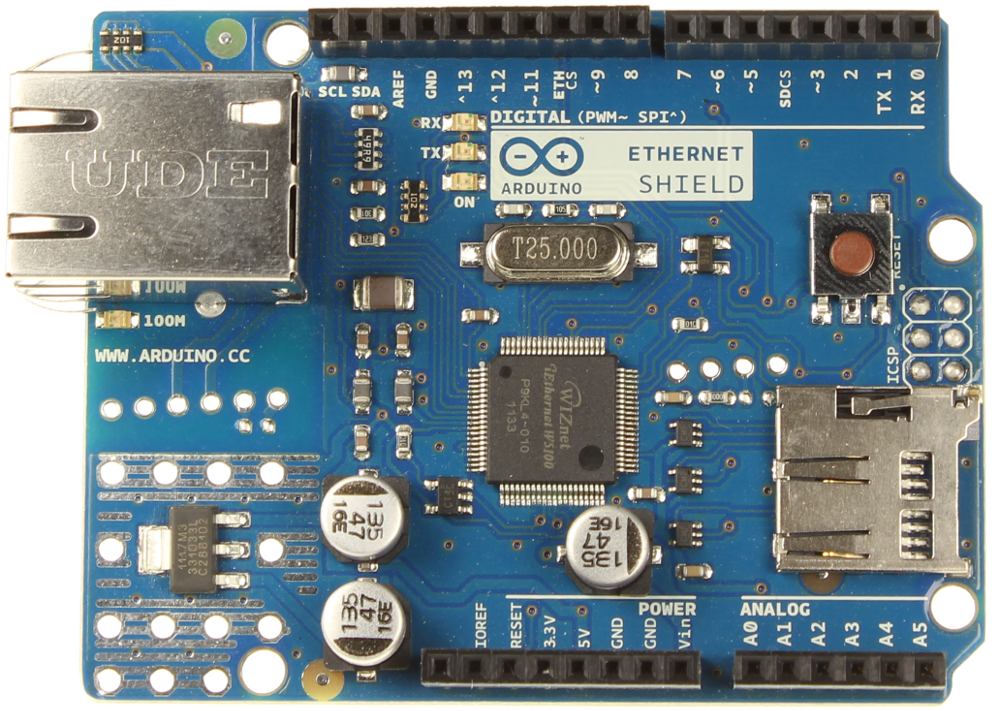
\includegraphics[width=70pt]{./img/shield_ethernet.png}
\end{center}
\end{column}
\end{columns}

\end{column}
\end{columns}




\end{frame}

% % % % % % % % % %
\begin{frame}{Onde buscar?}
\begin{itemize}
	\item http://arduino.cc
	\item http://arduino.cc/en/Tutorial/HomePage
	\item http://blog.bricogeek.com
	\item http://tallerarduino.com
	\item http://playground.arduino.cc/

\end{itemize}
\end{frame}




%%%%%%%%%%%%%%%%%%%%%%%%%%%%%%%%%%%%%%%%%%%%%%%%%%%%%%
\section{A cacharrear!}
\begin{frame}
\huge{\centerline{\textbf{\color{blue} \insertsection}}}
\end{frame}



% % % % % % % % % %
\begin{frame}{Blink}
\begin{description}
 \item[Esquema:] Sen esquema
 \item[Código:] Exemplos Básicos do Arduino IDE (Blink)
\end{description}
\end{frame}


% % % % % % % % % %
\begin{frame}{Lectura de potenciómetro}
\begin{center}
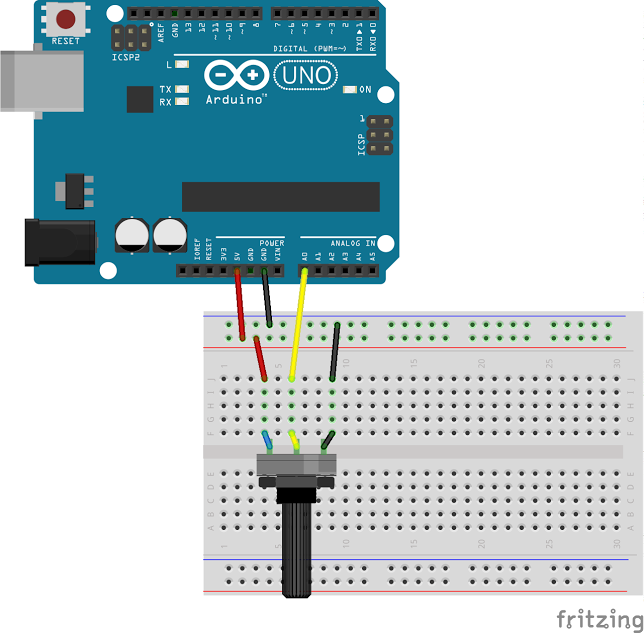
\includegraphics[width=165pt]{./img/lecturaPote.png}
\end{center}

\begin{description}
\item[Código:] Exemplos Básicos do Arduino IDE (analogReadSerial)
\end{description}
\end{frame}

% % % % % % % % % %
\begin{frame}{Saídas}
\begin{center}
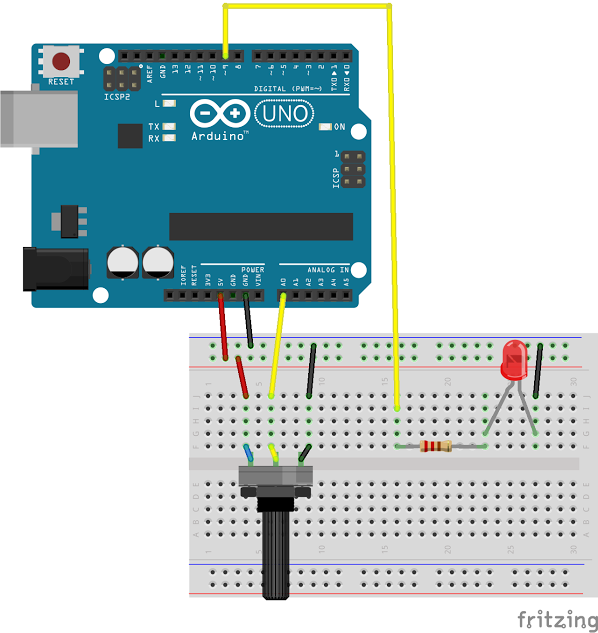
\includegraphics[width=170pt]{./img/esquemaPoteLed.png}
\end{center}

\begin{description}
\item[Código:] Exemplos Básicos do Arduino IDE (Fade)
\end{description}
\end{frame}


% % % % % % % % % %
\begin{frame}{Interaccionando}
\begin{description}
\item[Esquema:] O do exemplo anterior
\item[Código:] Fusión dos dous anteriores
\end{description}
\end{frame}

% % % % % % % % % %
\begin{frame}{Temperatura}
\begin{center}
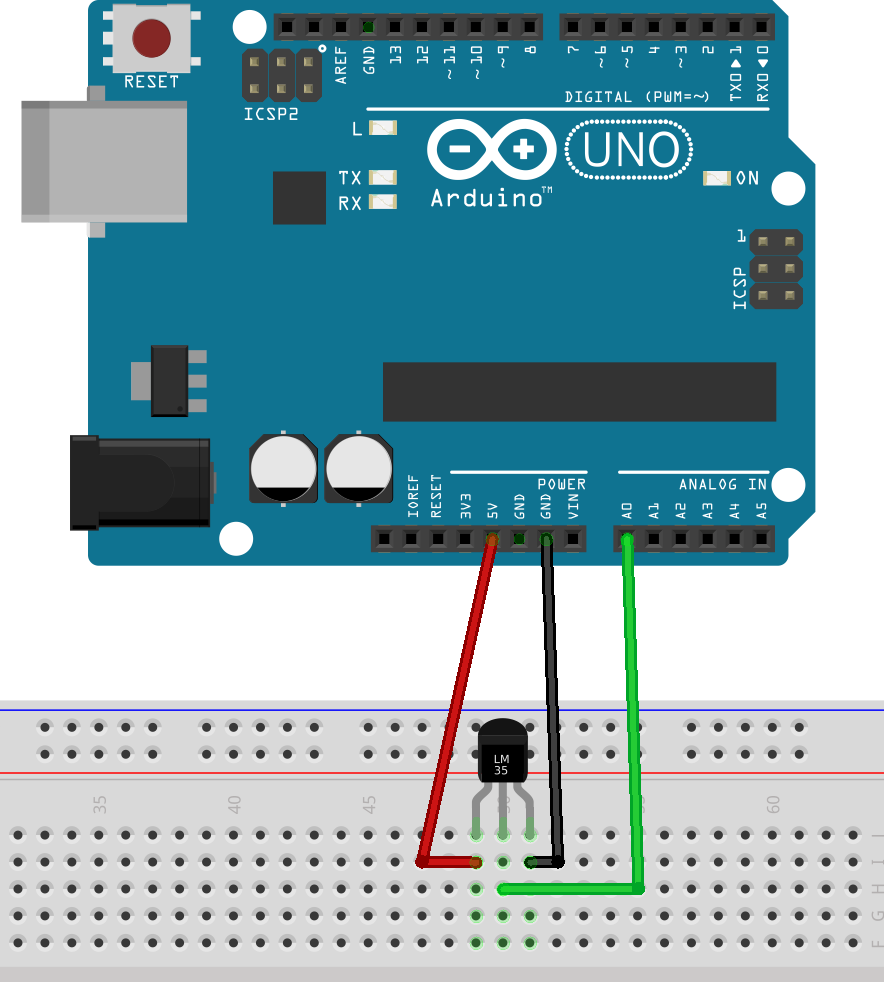
\includegraphics[width=160pt]{./img/esquema_temperatura.png}
\end{center}

\begin{description}
\item[Código:] Partimos do exemplos Básicos do Arduino IDE (analogReadSerial)
\end{description}
\end{frame}

% % % % % % % % % %
\begin{frame}{Alarma de Temperatura}
\begin{center}
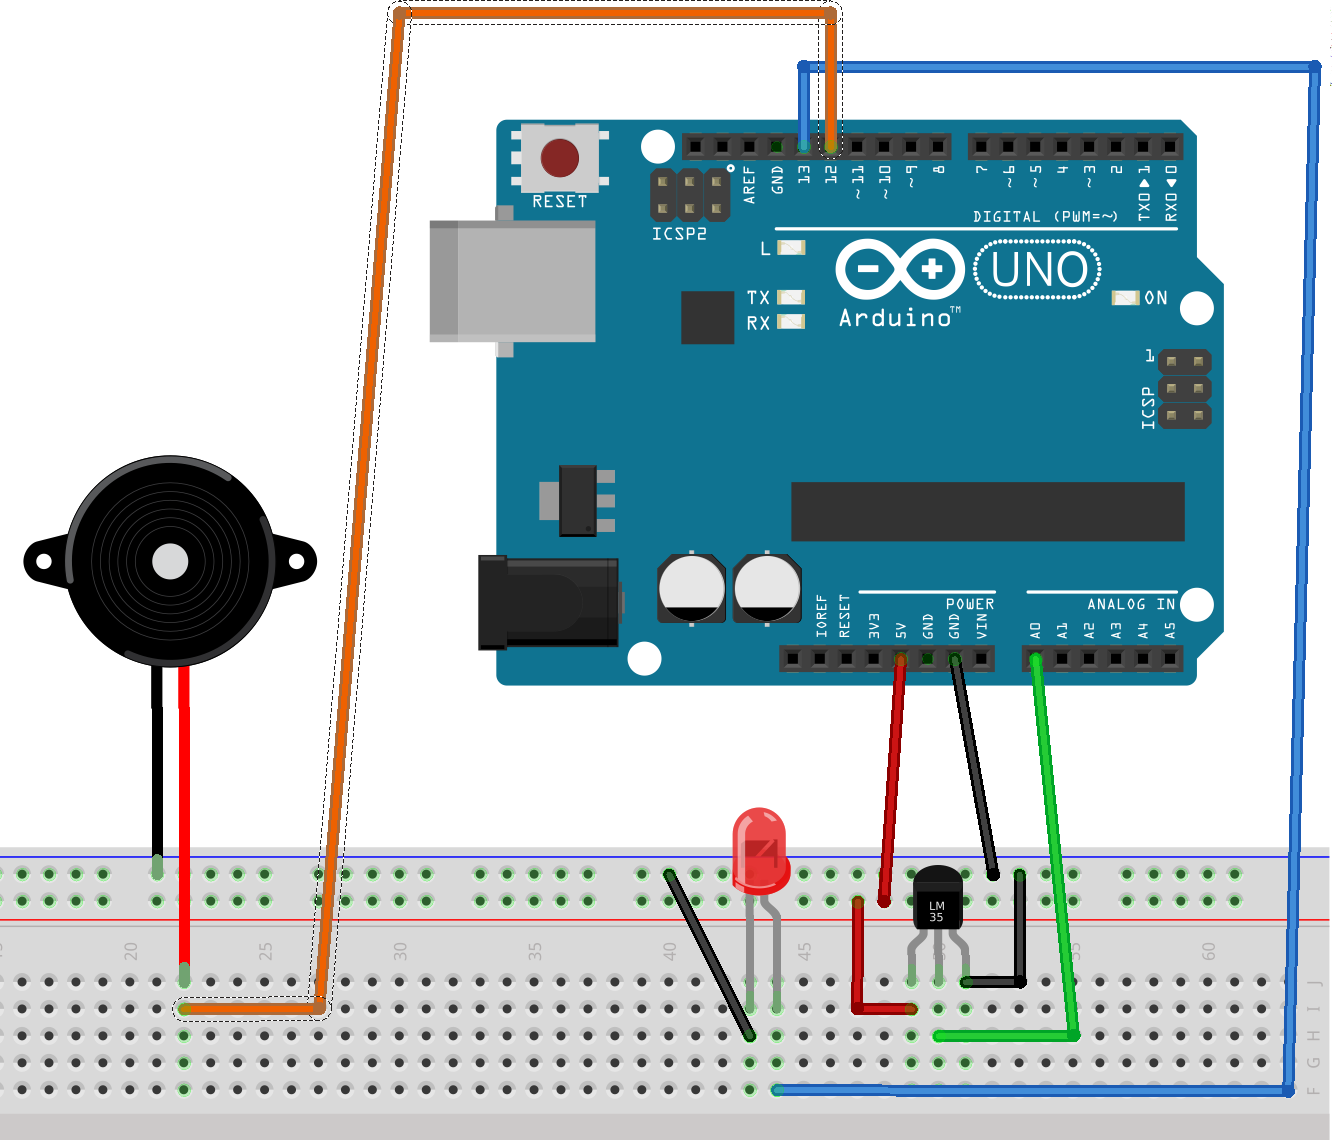
\includegraphics[width=160pt]{./img/esquema_temperatura_alarma.png}
\end{center}

\begin{description}
\item[Código:] Partimos do código anterior
\end{description}
\end{frame}

% % % % % % % % % %
\begin{frame}{Gardando datos en memoria EEPROM}
\begin{description}
\item[Esquema:] O do exemplo anterior
\item[Código:] Partimos dos exemplos EEPROM do Arduino IDE e do código anterior
\end{description}
\end{frame}

% % % % % % % % % %
\begin{frame}{Música no Arduino}

\end{frame}





%%%%%%%%%%%%%%%%%%%%%%%%%%%%%%%%%%%%%%%%%%%%%%%%%%%%%%
\section{Máis cousas}


% % % % % % % % % %
\begin{frame}{Dúbidas, comentarios...}

\end{frame}

\end{document}
